The 2 digit 7 segment display is used for different purposes depending on the mode and selected function as shown below. There are three distinct types of information: display of numeric values (parameters values), scrolling of (short) texts, indicator symbols for pick-me-up in Preset Panel mode, etc.

\scalebox{0.35}{
  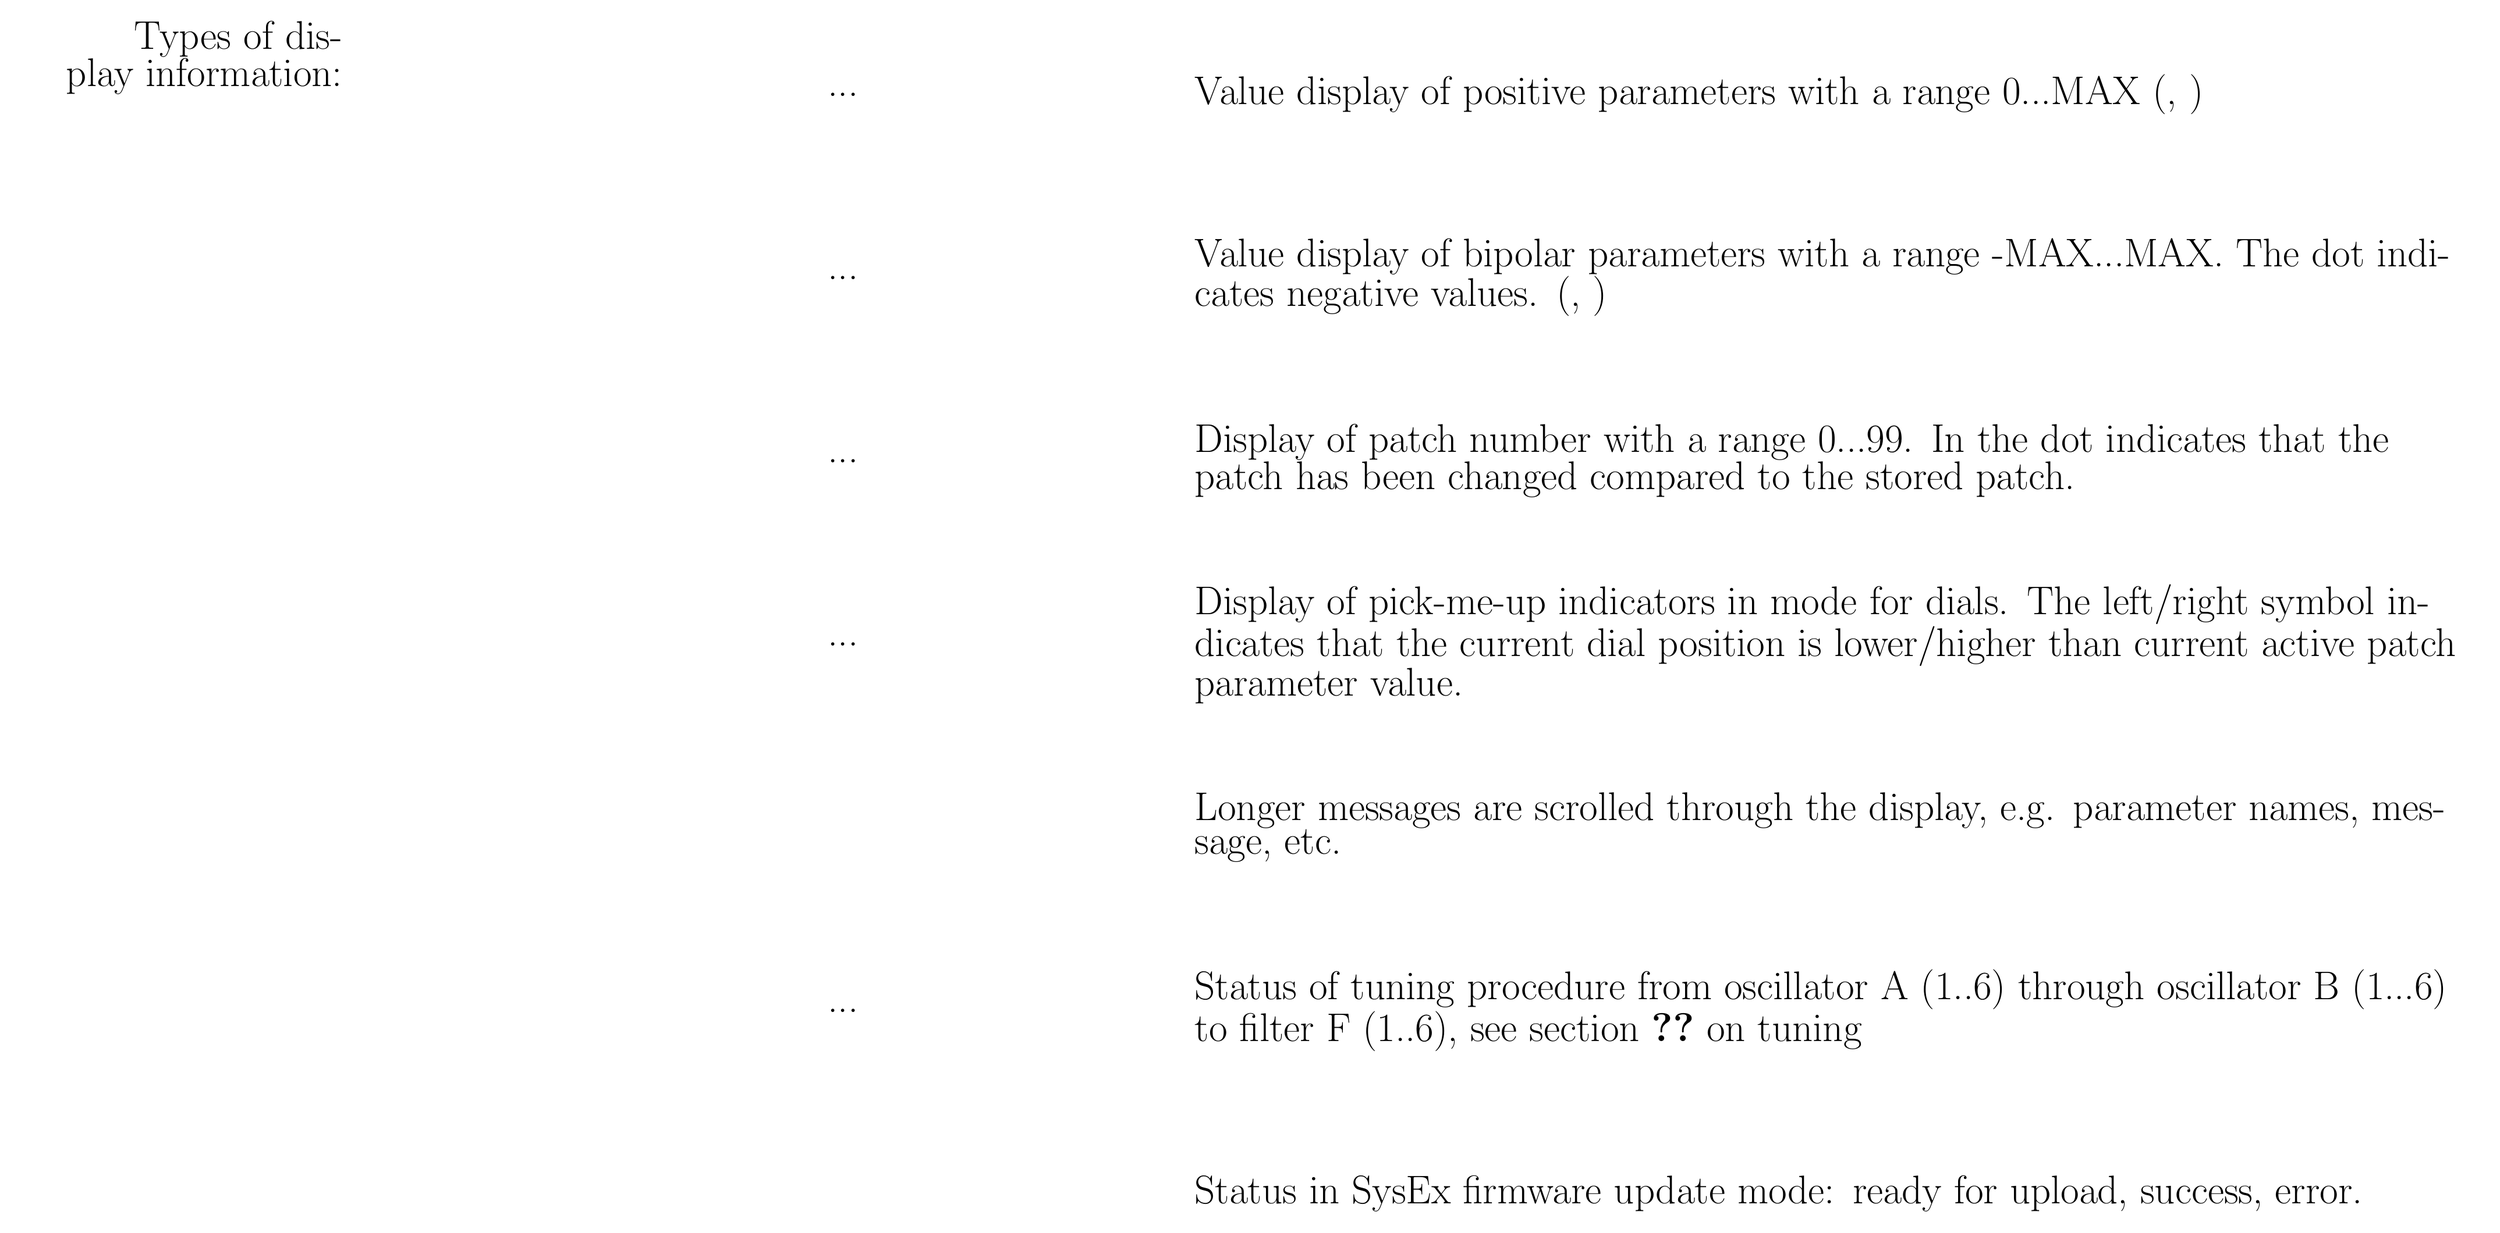
\begin{tikzpicture}[scale=0.8]
  \node[font=\fontsize{26}{12}\selectfont, align=right, outer sep=0.5mm, anchor = west, text width=7cm] at (-8cm,21.0cm) {Types of display information:};
    
    \prophetdisplay{9.5cm,20cm}{123456}{123456}{}
    \prophetdisplay{18cm,20cm}{123467}{123467}{}
    \node[font=\fontsize{26}{12}\selectfont, align=left, outer sep=0.5mm, anchor = west, text width=28cm] at (14cm,20cm) {...};
    \node[font=\fontsize{26}{12}\selectfont, align=left, outer sep=0.5mm, anchor = west, text width=28cm] at (24cm,20cm) {Value display of positive parameters with a range 0...MAX (\livemode, \presetpanel)};
    
    \prophetdisplay{9.5cm,15cm}{13467}{123456}{1}
    \prophetdisplay{18cm,15cm}{13467}{123456}{}
    \node[font=\fontsize{26}{12}\selectfont, align=left, outer sep=0.5mm, anchor = west, text width=28cm] at (14cm,15cm) {...};
    \node[font=\fontsize{26}{12}\selectfont, align=left, outer sep=0.5mm, anchor = west, text width=28cm] at (24cm,15cm) {Value display of bipolar parameters with a range -MAX...MAX. The dot indicates negative values. (\livemode, \presetpanel)};

    \prophetdisplay{9.5cm,10cm}{13467}{23}{}
    \prophetdisplay{18cm,10cm}{13467}{23}{1}
    \node[font=\fontsize{26}{12}\selectfont, align=left, outer sep=0.5mm, anchor = west, text width=28cm] at (14cm,10cm) {...};
    \node[font=\fontsize{26}{12}\selectfont, align=left, outer sep=0.5mm, anchor = west, text width=28cm] at (24cm,10cm) {Display of patch number with a range 0...99. In \presetpatch the dot indicates that the patch has been changed compared to the stored patch.};

    \prophetdisplay{9.5cm,5cm}{567}{}{}
    \prophetdisplay{18cm,5cm}{}{237}{}
    \node[font=\fontsize{26}{12}\selectfont, align=left, outer sep=0.5mm, anchor = west, text width=28cm] at (14cm,5cm) {...};
    \node[font=\fontsize{26}{12}\selectfont, align=left, outer sep=0.5mm, anchor = west, text width=28cm] at (24cm,5cm) {Display of pick-me-up indicators in \presetpanel mode for dials. The left/right symbol indicates that the current dial position is lower/higher than current active patch parameter value.};

    \begin{scope}[xslant=0.1]
      \SSGBit[1.0cm]{0cm,0cm}{456}
      \SSGBit[1.0cm]{1.6cm,0cm}{1567}
      \SSGBit[1.0cm]{3.2cm,0cm}{3457}
      \SSGBit[1.0cm]{4.8cm,0cm}{}
      \SSGBit[1.0cm]{9.7cm,0cm}{357}
      \SSGBit[1.0cm]{11.3cm,0cm}{457}
      \SSGBit[1.0cm]{12.9cm,0cm}{}
      \SSGBit[1.0cm]{14.5cm,0cm}{47}
      \SSGBit[1.0cm]{16.1cm,0cm}{}
      \SSGBit[1.0cm]{17.7cm,0cm}{3457}
      \SSGBit[1.0cm]{19.3cm,0cm}{1567}
      \SSGBit[1.0cm]{20.9cm,0cm}{1567}
    \end{scope}
    \prophetdisplay{6.4cm,0cm}{13467}{2367}{}
    \node[font=\fontsize{26}{12}\selectfont, align=left, outer sep=0.5mm, anchor = west, text width=28cm] at (24cm,0cm) {Longer messages are scrolled through the display, e.g. parameter names, message, etc.};

    \prophetdisplay{9.5cm,-5cm}{123567}{23}{}
    \prophetdisplay{18cm,-5cm}{1567}{23}{}
    \node[font=\fontsize{26}{12}\selectfont, align=left, outer sep=0.5mm, anchor = west, text width=28cm] at (14cm,-5cm) {...};
    \node[font=\fontsize{26}{12}\selectfont, align=left, outer sep=0.5mm, anchor = west, text width=28cm] at (24cm,-5cm) {Status of tuning procedure from oscillator A (1..6) through oscillator B (1...6) to filter F (1..6), see section \ref{tuning} on tuning};

    \prophetdisplay{8cm,-10cm}{23456}{}{}
    \prophetdisplay{13cm,-10cm}{13467}{}{}
    \prophetdisplay{18cm,-10cm}{14567}{}{}
    \node[font=\fontsize{26}{12}\selectfont, align=left, outer sep=0.5mm, anchor = west, text width=28cm] at (24cm,-10cm) {Status in SysEx firmware update mode: ready for upload, success, error.};
  \end{tikzpicture}
}

Note that while numeric values are shown in the range -50 to 50 or 0 to 99, the internally used accuracy and dial sensitivity is much higher. As a result of this, noticeable patch changes can be achieved by turning a dial slightly while the display continues to show the same value. The display is a rough indication of the current values. However, it can be used accurately when centering bipolar dials.
